% This is samplepaper.tex, a sample chapter demonstrating the
% LLNCS macro package for Springer Computer Science proceedings;
% Version 2.20 of 2017/10/04
%
\documentclass[runningheads]{llncs}
%
\usepackage{graphicx}
% Used for displaying a sample figure. If possible, figure files should
% be included in EPS format.
%
% If you use the hyperref package, please uncomment the following line
% to display URLs in blue roman font according to Springer's eBook style:
% \renewcommand\UrlFont{\color{blue}\rmfamily}

\begin{document}
%
\title{Simplex vs. Montecarlo, a brief comparision.\thanks{Supported by Universidad Tecnológica de Pereira.}}
%
%\titlerunning{Abbreviated paper title}
% If the paper title is too long for the running head, you can set
% an abbreviated paper title here
%
\author{Oscar Eduardo Bernal}
%
\authorrunning{O. Bernal}
% First names are abbreviated in the running head.
% If there are more than two authors, 'et al.' is used.
%
\institute{Universidad Tecnológia de Pereira, Colombia
\email{}}
%
\maketitle              % typeset the header of the contribution
%
\begin{abstract}
The Monte Carlo Method give us a process to solve big problems using randomness, by other side simplex is a method to solve linear optimization ploblems through an iterative process. Using HPC we can have an approach to parallel computing with a good amount of threads, but the Simplex method can't be easily parallelizable because in each iteration it depends of the previous state, while using Monte Carlo each step of the process is completely independient. Even so the question arises, is there really a difference between the Simplex method and the Monte Carlo method in a high-performance environment to solve linear optimization ploblems?

\keywords{HPC \and linear optimization \and Monte Carlo \and parallel computing \and Simplex}
\end{abstract}
%
%
%
\section{Introduction}
Es facil pensar en que un algoritmo puede ser mejor que otro, en especial cuando se trata de hacer tareas en paralelo, pero para poder lograr una comprension real de las implicaciones de una afirmación como esta se requiere, no solo un entendimiento de los algoritmos, si no tambien realizar un proceso de experimentacion, donde se pueda comprobar con datos reales la hipotesis planteada.

\subsection{Linear Optimization}
La optimizacion Lineal, tambien conocida como Programacion Lineal, y es el campo de la Optimizacion que se encarga de resolver problemas donde el objetivo es maximizar una funcion sujeta a una serie de restricciones expresadas mediante inecuaciones lineales. 

\subsection{Simplex Method}
El metodo Simplex es un metodo iterativo, que es usado por excelencia en el campo de la Optimizacion Lineal, se comporta como un algoritmo de pivote y va recorriendo los vertices de un poliedro n-dimensional, siendo n el numero de variables.

\subsection{Monte Carlo Method}
El metodo Monte Carlo es un metodo no determinista, que se utiliza para la aproximacion de problemas matematicos complejos y computacionalmente costos. Tiene su fundamento en la aleatoriedad mediante la cual va generando puntos que se evaluan y determinan posibles soluciones.

\subsection{Parallel computing}
La computacion paralela es la forma de computo en la que muchas instrucciones son ejecutadas simultaneamente, parte del principio de que los grandes problemas a menudo se pueden dividir en problemas mas pequeños y resolver individualmente.

\subsection{Hipotesis}
Teniendo en cuenta la informacion sobre los dos metodos que se abordan en este documento se plantea la siguient hipotesis: 
Montecarlo es mejor que el metodo Simplex para solucionar problemas de Optimizacion Lineales con un gran numero de variables.

\section{Implementation}
Para poder poner a prueba esta hipotesis se desarrollaron 3 implementaciones, la primera y mas basica es una implementacion secuencial del metodo simplex, la segunda es una implementacion lineal del metodo montecarlo, y la ultima una version concurrente del metodo montecarlo.

\subsection{Sequential Simplex Method}
El metodo Simplex parte de una matriz nxm donde n es el numero de variables del problema y m es el numero de restricciones, sobre esta matriz se empieza a iterar cambiando los valores de ciertas filas y columnas en cada iteracion, hasta que se encuentra la solucion.
Este metodo tiene una complejidad algoritmica de orden cuadrado O(n2)­ en el peor de los casos, y en el mejor una complejidad de orden lineal (n+m)

\subsection{Sequential Monte Carlo Method}
El metodo Monte Carlo en su version secuencial realiza un numero fijo de pasos, que para este estudio es de 21.474.836, en los cuales genera n numeros aleatorios y luego realiza m+1 validaciones (siendo n y m el numero de variables y de restricciones respectivamente), para determinar si estos numeros cumplen con las condiciones del algoritmo, este ciclo se realiza multiples veces, obteniendo cada vez distintos valores guardando unicamente el estado para el cual el problema de optimizacion lineal es maximo.
Este metodo tiene una complejidad algoritmica de orden lineal O(n) en cualquier caso, ya que sin importar el resultado el se ejecuta un numero fija de veces, que no aumenta ni disminuye. 

\subsection{Parallel Monte Carlo Method}
La implementacion paralela del metodo de Monte Carlo crea una cantidad fija de hilos en cada bloque, que para este caso son 1024, y una rejilla de 1024 bloques, se utiliza una estructura lineal tanto para la distribucion de la rejilla asi como para la del bloque, para facilitar la comprension del algoritmo, pero esta se puede ampliar a una estructura tridimensional sin mayor problema.
\paragraph{}
El Kernel de este metodo se comporta de forma similar a su predecesor secuancial, probando distintas combinaciones de numeros aleatorios, y guardando en una matriz el estado del minimo encontrado, para luego de forma secuencial recorrer esta matriz para encontrar el valor minimo de todos, este recorrido no se hace de la totalidad de la matriz, si no de una sola posicion de la matriz, quedando de esta forma con complejidad lineal para el Kernel y lineal tambien para la determinacion del menor.

\section{Results}
Luego de ejecutar los metodos implementados para problemas de optimizacion con diferentes numeros de variables y restricciones, se encontro que los tiempos de ejecucion no resultaron como se esperaba, aunque el comportamiento de los algoritmos corresponde con el orden de complejidad, la magnitud de los tiempos demuestra la importancia de la experimentacion.
\paragraph{}
Asi se tiene que aunque el metodo Simplex tiene una complejidad de orden cuadrado, esto es unicamente en el peor de los casos y este es un caso extraño, ya que en la mayoria de problemas el caso mas comun es de orden lineal, causando asi tiempos de ejecucion menores que la ejecucion de Monte Carlo, que se comporta igualmente con orden lineal pero con un tiempo inicial mayor.

\begin{figure}
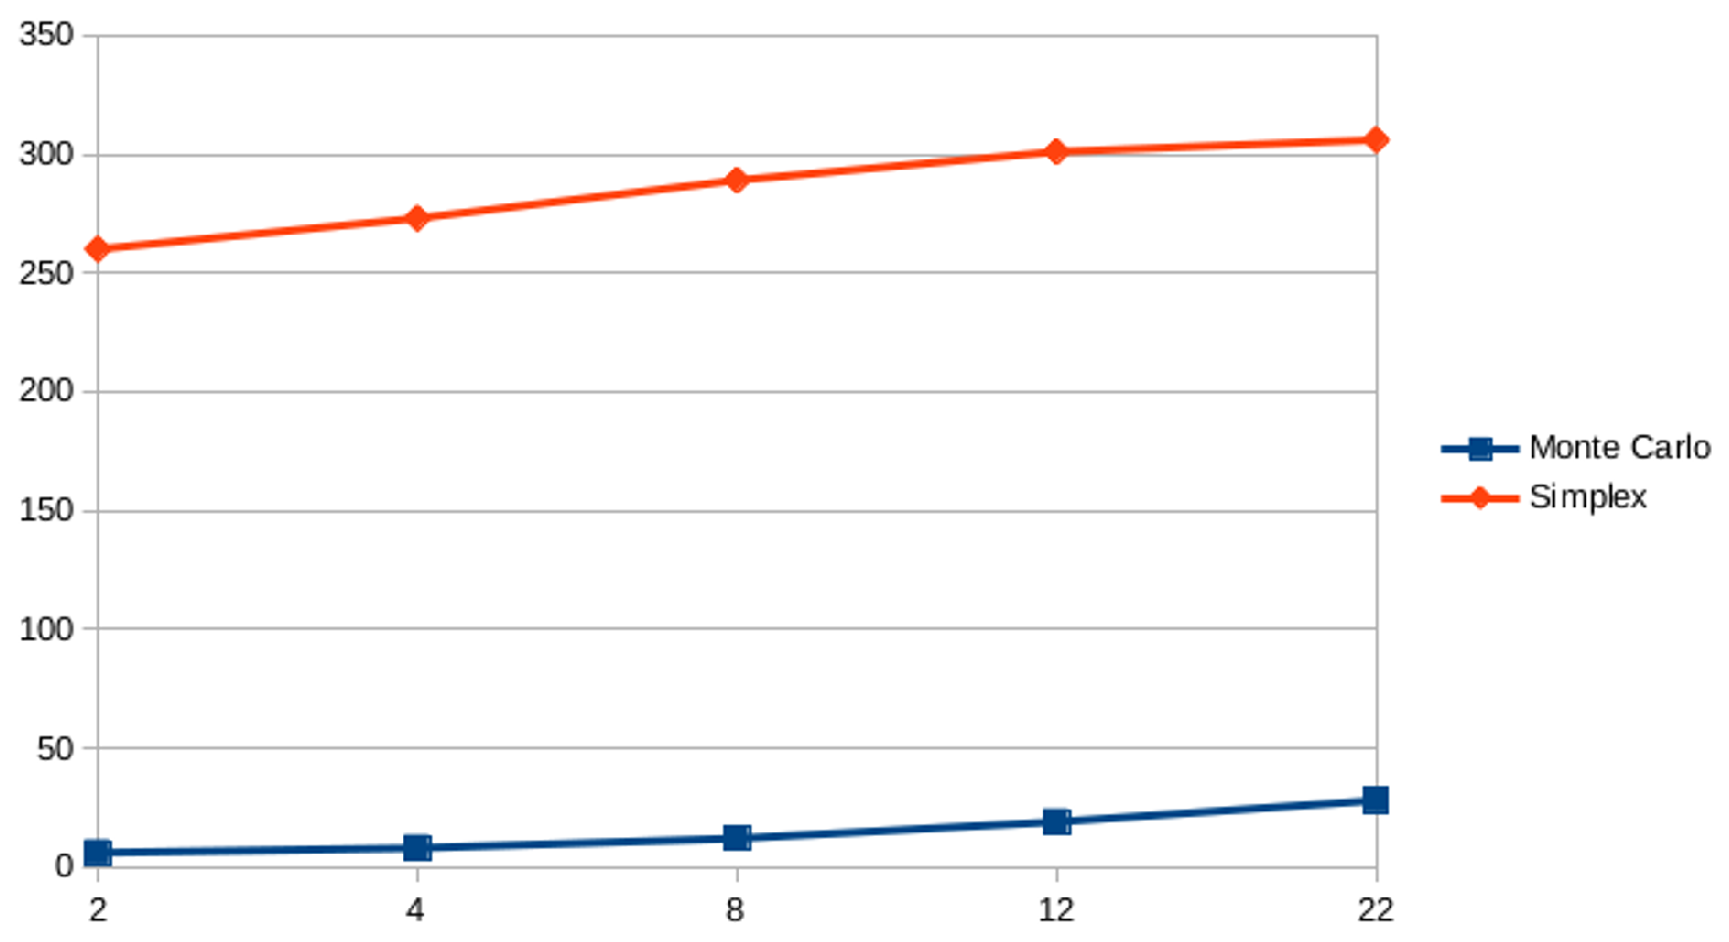
\includegraphics[width=\textwidth]{fig1.eps}
\caption{A figure caption is always placed below the illustration.
Please note that short captions are centered, while long ones are
justified by the macro package automatically.} \label{fig1}
\end{figure}

Adicionalmente se observo, durante la toma de datos, que dificilmente se encuentran problemas de optimizacion lineal de un gran numero de variables, el problema de mayor tamaño encontrado fue de 8 variables, todos los demas problemas se construyeron artificialmente para probar el comportamiento de los metodos. El valor mas grande probado fue de 22 variables y 23 restricciones. 
\paragraph{}
El metodo Monte Carlo, a diferencia del metodo Simplex, encuentra valores cercanos o aproximados a la respuesta esperada, no siempre el valor exacto, y en esto el Metodo Simplex puede llevarle tambien una ventaja, pero esto solo ocurre en los casos en los que es problema tiene una solucion unica. En los casos en que esto no es asi, el metodo Monte Carlo encuentra una solucion factible, en lugar de bloquearse como el metodo simplex.  
\paragraph{}
Para problemas de optimizacion no lineales el metodo Monte Carlo se puede adaptar con pocos cambios y conservando sus propiedades, mientras que el metodo simplex se hace inutil y se requieren dintintos metodos que cambian dependiendo del tipo de problema.

\section{Conclusions}
\paragraph{}
No siempre paralelo es mejor, es facil pensar que al utilizar una alternativa paralela para la solucion de un problema se pueden obtener mejores resultados, pero esto siempre depende de la naturaleza del problema y es necesario realizar un correcto analisis para determinar si la implementacion de un metodo paralelo es la mejor opcion.
\paragraph{}
El orden de complejidad de un algoritmo es una gran ayuda para conocer el posible desempeño del mismo, pero se debe tener tambien en cuenta el comportamiento comun del mismo, ya que existe la posibilidad que el caso comun no sea el peor de los casos.
\paragraph{}
En todo proceso de experimentacion es importante tener claramente definida la hipotesis y realizar un buen analisis del problema, pero tambien prestar mucha atencion a los resultados, ya que no siempre el resultado sera e esperado y es importante determinar el porque de estos resultados.
\paragraph{}
La computacion de alto rendimiento es una tecnologia que brinda muchas posibilidades, pero como cualquier tecnologia debe utilizarse responsablemente y su capacidad dependera de la formulacion y la implementacion de las algoritmos que se desarrollen para ella. 
\paragraph{}
El metodo Monte Carlo se presta para resolver toda una gama de problemas diferentes, mientras que el metodo simplex se especializa en una sola clase de problemas y resulta ser muy optimo. De esta forma se puede concluir que una solucion general no siempre es la mejor alternativa, a veces es mejor tener soluciones optimzadas a los requerimientos del problema. 

%
% ---- Bibliography ----
%
% BibTeX users should specify bibliography style 'splncs04'.
% References will then be sorted and formatted in the correct style.
%
% \bibliographystyle{splncs04}
% \bibliography{mybibliography}
%
%\begin{thebibliography}{8}
%\bibitem{ref_article1}
%Author, F.: Article title. Journal \textbf{2}(5), 99--110 (2016)
%
%\bibitem{ref_lncs1}
%Author, F., Author, S.: Title of a proceedings paper. In: Editor,
%F., Editor, S. (eds.) CONFERENCE 2016, LNCS, vol. 9999, pp. 1--13.
%Springer, Heidelberg (2016). \doi{10.10007/1234567890}
%
%\end{thebibliography}

\end{document}
